\paragraph{Sơ đồ tuần tự luồng đánh dấu cuộc trò chuyện}

Luồng nghiệp vụ này mô tả
quy trình người dùng thực hiện đánh dấu (bookmark)
một cuộc trò chuyện và đính kèm ghi chú cá nhân.

\begin{figure}[H]
\centering
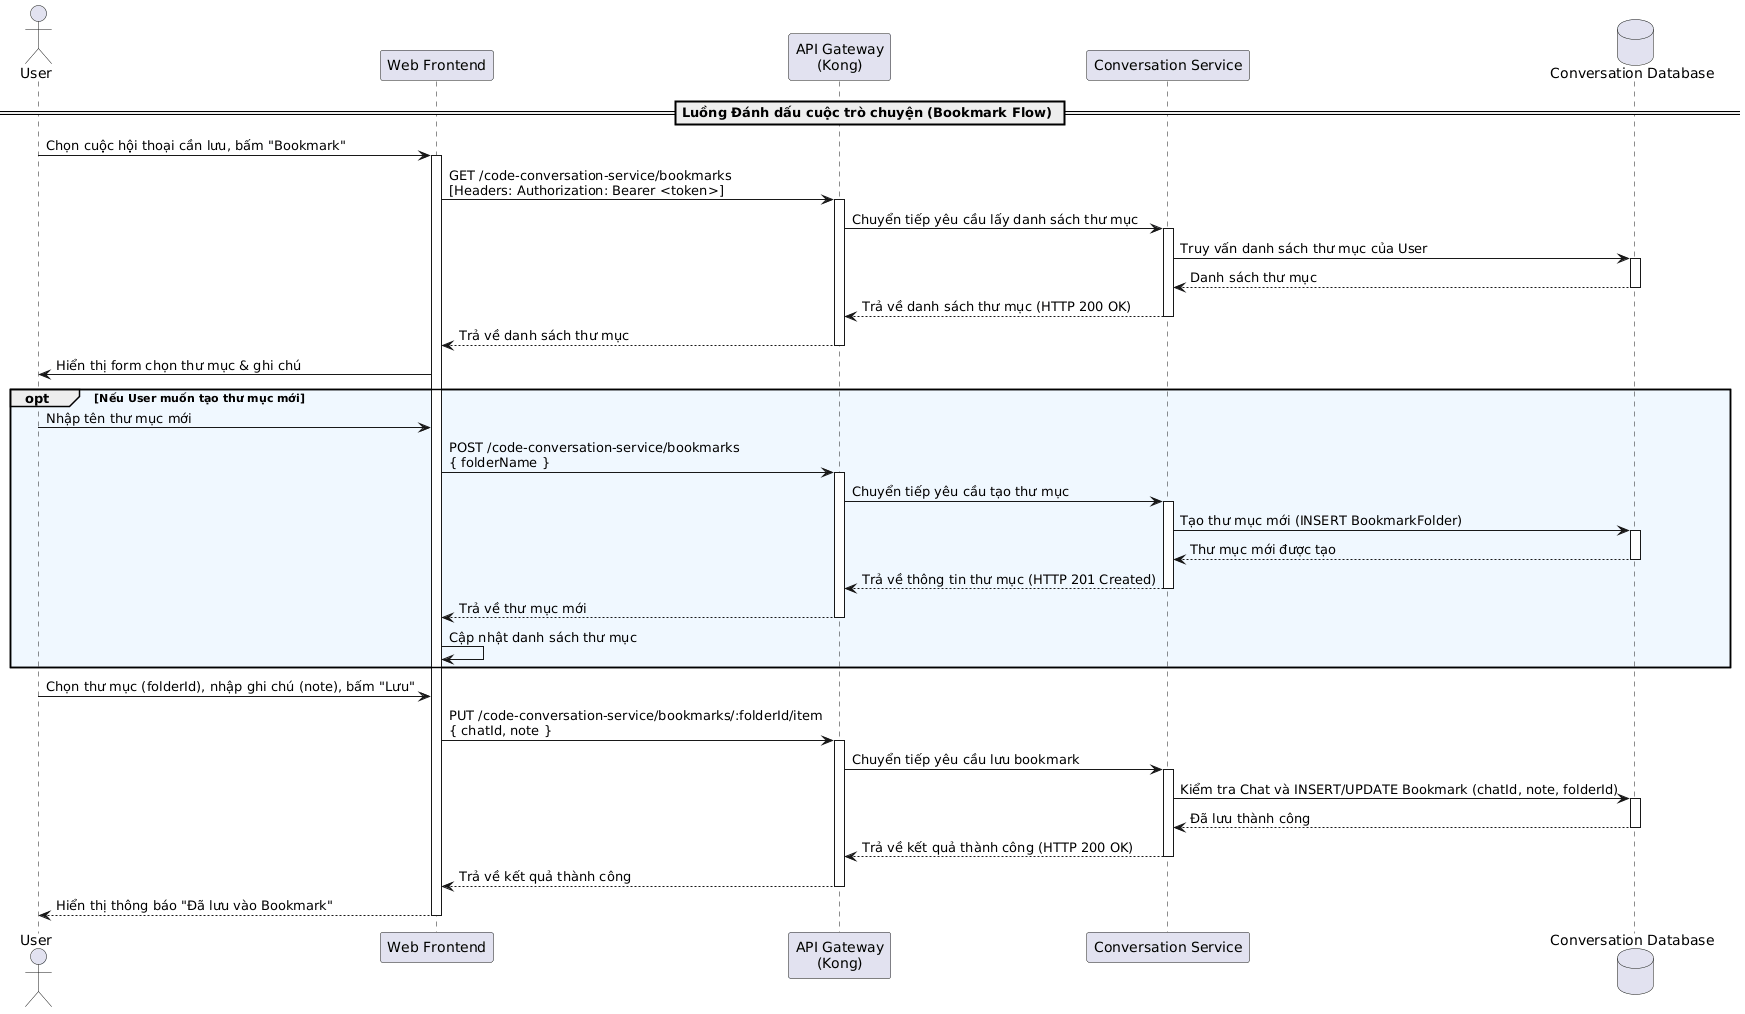
\includegraphics[width=0.95\textwidth]{contents/Sequence/UML-Sequence-UserBookmarkChat.png}
\caption{Sơ đồ tuần tự luồng đánh dấu cuộc trò chuyện}
\end{figure}

\begin{table}[H]
\centering
\renewcommand{\arraystretch}{1.3}

\begin{tabular}{|l|l|p{5cm}|}
\hline
\textbf{Thành phần} & \textbf{Phân loại} & \textbf{Vai trò trong hệ thống} \\ \hline
User & Actor & Người dùng chọn cuộc trò chuyện cần lưu trữ và ghi chú thêm. \\ \hline
Web Frontend & Component & Giao diện web Next.js. \\ \hline
API Gateway (Kong) & Component & Cổng API chuyển tiếp các yêu cầu API. \\ \hline
Conversation Service & Microservice & Tiếp nhận yêu cầu lấy danh sách thư mục, tạo thư mục mới và liên kết cuộc trò chuyện vào thư mục bookmark. \\ \hline
Conversation Database & Database & Lưu trữ các thư mục bookmark (BookmarkFolder) và các bản ghi liên kết bookmark (Bookmark) của người dùng. \\ \hline
\end{tabular}
\caption{Các thành phần tham gia luồng đánh dấu cuộc trò chuyện}
\end{table}

\subparagraph{Mô tả tổng quan}

\begin{itemize}

\item \textbf{Yêu cầu danh sách thư mục:}
Khi người dùng chọn đánh dấu
cuộc trò chuyện trên giao diện,
giao diện gửi yêu cầu lấy danh sách thư mục lưu trữ hiện có
của người dùng để hiển thị lên màn hình.

\item \textbf{Tạo thư mục mới (nếu cần):}
Nếu người dùng muốn tạo thư mục mới,
người dùng nhập tên thư mục
và giao diện gửi yêu cầu tạo thư mục.
Hệ thống lưu thư mục mới
vào CSDL trò chuyện
và cập nhật lại danh sách hiển thị.

\item \textbf{Lưu thông tin đánh dấu:}
Người dùng chọn thư mục lưu trữ,
điền ghi chú cá nhân và nhấn lưu.
Giao diện gửi yêu cầu đính kèm cuộc trò chuyện
vào thư mục đã chọn kèm ghi chú.

\item \textbf{Cập nhật CSDL:}
Dịch vụ trò chuyện kiểm tra sự tồn tại
của cuộc trò chuyện
và thực hiện lưu hoặc
cập nhật thông tin đánh dấu vào CSDL trò chuyện,
sau đó trả về thông báo thành công
để cập nhật giao diện của người dùng.

\end{itemize}
